%  Robotics Text  by Jacob Rosen and Blake Hannaford
% (c) 2007  Jacob Rosen and Blake Hannaford
%

\chapter{Mechatronics and Design of Manipulators}

\section{Problem Statement and Learning Objectives}
% Problem Statement and Learning Objectives for Chapter 10

\paragraph{Problem Statement}
 This chapter considers some aspects of design of serial link mechanisms for manipulation.

\paragraph{Learning Objectives}
Upon completing this Chapter, the reader should be able to
\begin{itemize}
  \item 
\end{itemize}
%
% I'm worried that this chapter will have to be too superficial.  Maybe an example with one or two DOF but actual implementation??

\section{Sensors}

\subsection{Force Sensors}

%%%%** Section 1.1
\paragraph{Load Cell}
\begin{indent}
A {\bf ``Load Cell" } is a structure which supports the load
and deflects a known amount in response to applied forces
and torques.  The deflections are measured to characterize
the applied forces and torques.
\end{indent}

%\end{slide}
%\begin{slide}

\paragraph{Example: Cantilever Beam}

%%%%** Figure 1
\begin{figure}[ht]	%<!s>
\begin{center}
\scalebox{1}{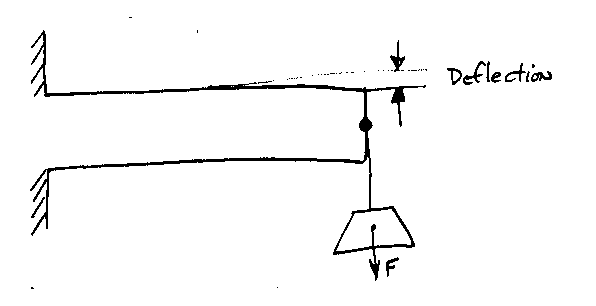
\includegraphics{figs10/00102.eps}}	%<hn>
%\scalebox{1}{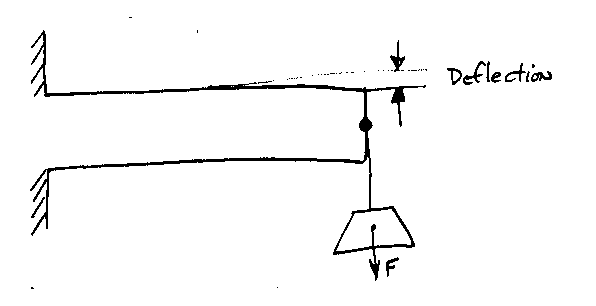
\includegraphics{figs10/00102.eps}}
\caption{Cantilever Beam.  When load $F$ is applied	%<!s>
to the end of the beam, the beam deflects a known amount. }	%<!s>
\end{center}
\end{figure}	%<!s>


%\end{slide}
%\begin{slide}
%%%%** Section 1.2
\paragraph{Stress and Strain}

%%%%** Section 1.2.1
\subsubsection{Stress}

\begin{itemize}

\item Stress ($\sigma$):  Force per unit area in one dimension.
\[
\sigma = \frac{F}{A}
\]
Units:  Pascals = $\frac {N}{M^2}$, psi.

\item Stress can be refered to as ``Compressive" (tending to compress	%<hn>
the material)and ``Tensile" (tending to elongate it).	%<hn>

%\item
%%%%** Figure 2
\begin{figure}[ht]	%<!s>
\begin{center}
\scalebox{1}{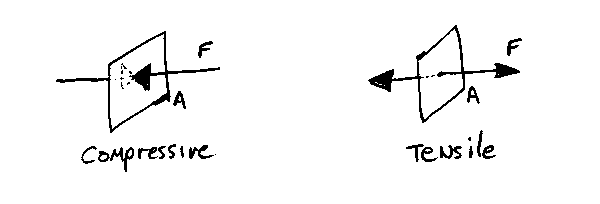
\includegraphics{figs10/00103.eps}}	%<hn>
%\scalebox{1}{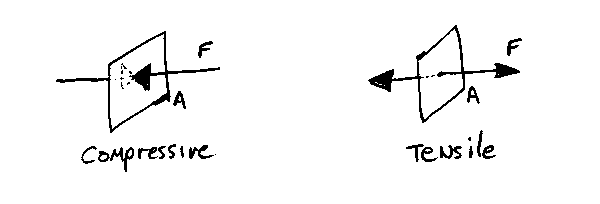
\includegraphics{figs10/00103.eps}}
\caption{Illustrations of Compressive and Tensile stress through a	%<!s>
 patch of area A. }	%<!s>
\end{center}
\end{figure}	%<!s>


\item Shear stress
refers to forces {\it in} the plane.  Shear stress can cause material to tear.	%<!s>
%%%%** Figure 3
\begin{figure}[ht]	%<!s>
\begin{center}
\scalebox{1}{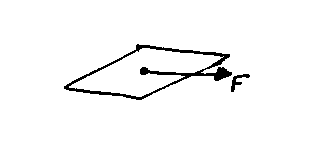
\includegraphics{figs10/00104.eps}}	%<hn>
%\scalebox{2}{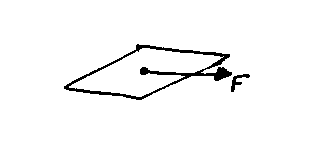
\includegraphics{figs10/00104.eps}}
\caption{Shear stress.  Shear stress is due to forces in the  plane. }	%<!s>
\end{center}
\end{figure}	%<!s>

\item 3-Dimensions:
 Full analysis of stress in 3-dimensions is complex and requires notion of	%<!s>
{\it Stress Tensor} --- a $3\times$3 matrix giving
the complete state of stress at a given point in the material.


\end{itemize}



%\end{slide}
%\begin{slide}

%%%%** Section 1.2.2
\subsubsection{Strain}

\begin{itemize}

\item  Strain, ($\epsilon$), is relative deformation.

\item 1 Dimension: Elongation Ratio
\[
\epsilon = \frac{\Delta L}{L}
\]

\item if $\frac{\Delta L}{L} = 10^{-5}$ we say ``10 micro-strain".

\item Strains of typical metal structures are very small
 (i.e. micro-strain).

\item Strains in biological tissues can be much larger
($\epsilon \approx 1$).

\item Advanced: Several Types of Strain


\end{itemize}

%%%%** Section 1.2.3
\subsubsection{Hooke's Law (Elastic Deformation)}
\[
\sigma = \mathrm{E}\epsilon
\]
where E is Young's Modulus.

\begin{itemize}

\item Biological materials rarely obey Hooke's Law.

\item Metals obey Hooke's Law very well for stresses below the
{\it elastic limit.}   If stress is greater, material
permanently deforms.

\end{itemize}

%\end{slide}
%\begin{slide}
%%%%** Figure 4
\begin{figure}[ht]	%<!s>
\begin{center}
\scalebox{1}{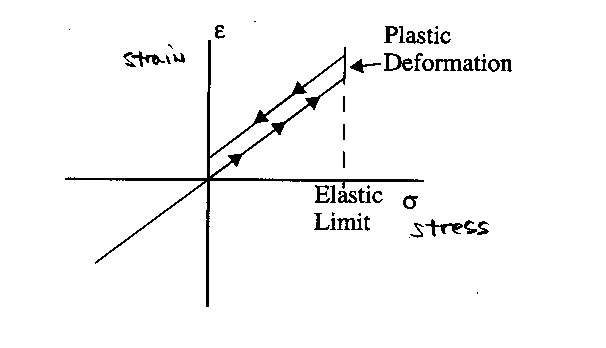
\includegraphics{figs10/00105.eps}}	%<hn>
%\scalebox{1.4}{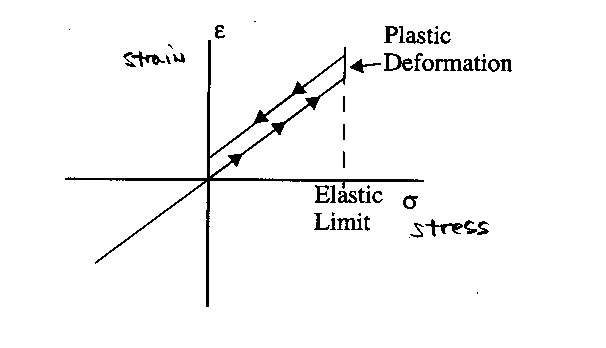
\includegraphics{figs10/00105.eps}}
\caption{Hookean behavior with Elastic Limit.  If stress increases	%<!s>
beyond Elastic Limit, material is permanently deformed. }	%<!s>
\end{center}
\end{figure}	%<!s>


%\end{slide}
%\begin{slide}
%%%%** Section 1.3
\paragraph{Cantilever Beam}

In this section we will analyze the basic cantalever beam (Figure \ref{cantaleverbeam}) so that we can make it into a force sensor.  Once we calculate the strain on the surface as a function of applied force, we can use a strain gauge to measure applied force.


%%%%** Figure 5
\begin{figure}[ht]	%<!s>
\begin{center}
\scalebox{1}{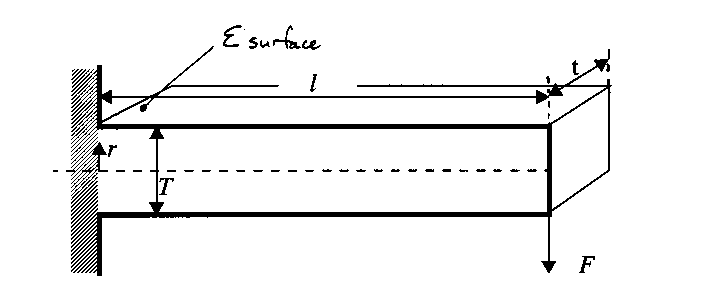
\includegraphics{figs10/00106.eps}}
\caption{ Rectangular cantilever beam is a simple load cell	%<!s>
structure for basic analysis. }\label{cantaleverbeam}
\end{center}
\end{figure}	%<!s>

	%<*hn>
We want to
derive $\epsilon_{surface}$	%<shn>
as a function of the applied
load, the dimensions of the beam, and the beam material's stiffness
(Young's modulus).  First, we assume that the beam is at static
equilibrium around the centerline along the wall.
The moment developed by the beam as it meets the wall is composed of forces produced by the elastic behavior of patches of the surface where the beam meets the wall.  Because of the way we apply force in Figure \ref{cantaleverbeam}, we can analyze these inifinitesimal patches as strips in the width direction (Figure \ref{cantaleverdetail}).

%%%%** Figure 5
\begin{figure}	%<!s>
\begin{center}
\includegraphics[width=5.0in]{figs10/00886.eps}
\caption{ Detail of the rectangular cantilever beam showing strips of constant stress. We integrate the moment due to each strip to get the total moment at equilibrium.}\label{cantaleverdetail}
\end{center}
\end{figure}	%<!s>

We equate the moment developed in the structure around the center line with the moment applied
by the external load.   As $\Delta r \to 0$, we integrate up the height of the beam and equate that moment to $F\times l$.

\[
F\times l = \int^{\frac{T}{2}}_{-\frac{T}{2}} r \sigma(r) t dr
\]
	%<*hn>
where r, t, F, l are defined in the figure, and $\sigma(r)$ is
the internal stress where the beam joins the wall.
Let us assume that $\sigma(r)$ varies linearly through the beam so
that
%Assume
	%<*>
\[
\sigma(r)= \alpha r
\]
where $\alpha$ is some positive constant.

%\end{slide}
%\begin{slide}


Then we have
\[
Fl = \alpha t \int^{\frac{T}{2}}_{-\frac{T}{2}} r^2 dr =
\frac{\alpha t T^3}{12}
\]


Solving for $\alpha$,
\[
\alpha = \frac{12l}{tT^3}F
\]
\[
\sigma(r)=\frac{12lr}{tT^3}F
\]

%\end{slide}
%\begin{slide}
Finally, we can evaluate $\sigma(r)$ at the surface
and use Young's modulus to convert stress to strain:
\[
\sigma(\frac{T}{2}) = \frac{12l\frac{T}{2}}{tT^3}F
\]
\[
= \frac{6l}{tT^2}F
\]
\[
\epsilon_{surface} = \frac{6l}{\mathrm{E}tT^2}F
\]

%\end{slide}
%\begin{slide}

%%%%** Section 1.4
\paragraph{Strain Gages}

(see {\tt http://www.measurementsgroup.com/guide/index.htm})

	%<*hn>
A strain gage is a device which transduces strain on a surface.
There are two types in common use, resistive metal foil, and semiconductor.
Both transduce strain by taking advantage of the variation of electrical
resistance with strain.

	%<*>
\paragraph{Metal Foil Strain Gages}

Metal foil gages are bonded to the surface and their resistance
changes in proportion to the surface strain.

%%%%** Figure 6
\begin{figure}[ht]	%<!s>
\begin{center}
\scalebox{1}{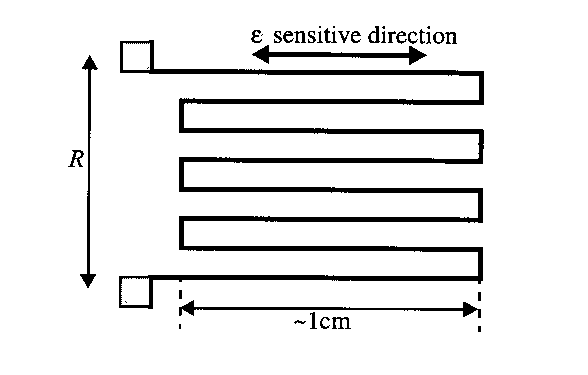
\includegraphics{figs10/00107.eps}}
\caption{ Diagram of a metal foil strain gage.  Conductor in the	%<!s>
 shape shown is attached to surface.   As surface deforms, conductive	%<!s>
 pattern changes length which changes resistance between contact pads (left).}	%<!s>
\end{center}
\end{figure}	%<!s>


%\end{slide}
%\begin{slide}

In simplified form,

\[
R = R_0 (1+\epsilon g)
\]

where $g = \frac{\Delta R}{R_0 \epsilon}$ is called the ``gage factor".
%
%Occasionally, the gage factor is not normalized by $R_0$ in which case
%it has the units of resistance, Ohms ($\Omega$), sometimes called
%``Ohms per strain".
	%<*>
For metal foil gages, $g \approx 3$.


%\end{slide}
%\begin{slide}

\paragraph{Semiconductor strain gages}

	%<*hn>
These are small chips of silicon with a single region of doping to
create a resistor. The chip is bonded to the load cell and its resistance
varies with strain. With a semiconductor strain gage, the designer
can expect signficantly higher gage factor of around
$g  \approx 150$.	%<*shn>



%%%%** Figure 7
\begin{figure}[ht]	%<!s>
\begin{center}
\scalebox{1.5}{
\includegraphics{figs10/00108.eps}}
\caption{ Diagram of a semiconductor strain gage. }	%<!s>
\end{center}
\end{figure}	%<!s>

%\end{slide}
%\begin{slide}

\paragraph{Properties of Strain Gages}
\begin{enumerate}
\item Very linear.  1\% is achievable due to Hooke's law.
Elastic limit must be avoided with a safety margin.

\item Wide dynamic range.  Example: Force/Torque sensor designed
by JPL for Space Shuttle RMS robot arm design range:  1N to $4 \times 10^5$N.
112db.

\item Temperature Sensitivity.  Both types are highly sensitive to temperature.

\item Interface between gage and structure requires care due to
different coefficients of thermal expansion between gage and structure.

	%<*hn>
\item Practicalities.  Foil gages are robust and cheap. Semiconductor
gages are delicate and expensive. Foil gages are fixed with an adhesive
which usually requires curing in an oven.  Semiconductor gages require
an elaborate process for attachment which must be done by a specialist.

% \item Practicalities:  Foil = cheap, robust.  \\
%Semiconductor = expensive, delicate, difficult to apply.
%
	%<*>
\end{enumerate}

%\end{slide}
%\begin{slide}


%%%%** Section 1.5
\paragraph{Temperature Sensitivity}
	%<*hn>
Careful thermal analysis is important for accurate force sensing
with strain gages. Two effects account for the temperature sensitivity
of metal foil strain gages:
	%<*>
\begin{itemize}
\item Thermal Coefficient of Resistance of gage material.
\item Difference in thermal coefficient of expansion of gage
and load cell structure.
\end{itemize}
	%<*hn>
The first causes resistance to change only as a function of temperature
and not of strain.  The second causes strains in the gage as a function
of temperature only.

The temperature dependence of the gage resistance can be described
by:
	%<*>
\[
r = \frac{\frac{\Delta R}{R_0}}{\Delta T} =
\beta_g + g \left (
    \frac{1+K_t}{1+\nu_0 K_t}
     \right )
     (\alpha_s - \alpha_g)
\]
Where

$\beta_g = $ thermal coefficient of resistance of the gage material.

$K_t$ = transverse sensitivity
 of the gage: the gage factor for strains	%<!s>
 orthogonal to the sensitive direction (extremely small for most	%<!s>
 gages and will be neglected).	%<!s>

$\nu_0$ = Poisson's ratio (typically 0.3)

$\alpha_s, \alpha_g$ = coefficients of thermal expansion of substrate and
gage respectively.

	%<*hn>
The first step to reduce temperature sensitivity is to make sure
the thermal expansion coefficients of the gage ($\alpha_g$)
and substrate ($\alpha_s$ ) are as close
as possible.
	%<*>

%\end{slide}
%\begin{slide}
We can then relate resistance to strain and temperature through
\[
R = R_0(1+g\epsilon)(1+r\Delta T)
\]


%\end{slide}
%\begin{slide}

	%<*hn>
The second step to compensating for the remaining temperature sensitivity
is to make a differential measurement of two gages which have the
same temperature but opposite strains.  In the case of a cantilever
beam, if we assume that the beam is at a uniform temperature, this
can be arranged by putting gages on either side of the beam. By
symmetry, $\epsilon_1 = -\epsilon_2$.

 \paragraph{Dual Gage beam}	%<*>
By symmetry, $\epsilon_1 = -\epsilon_2$.


%%%%** Figure 8
\begin{figure}[ht]	%<!s>
\begin{center}
\scalebox{1}{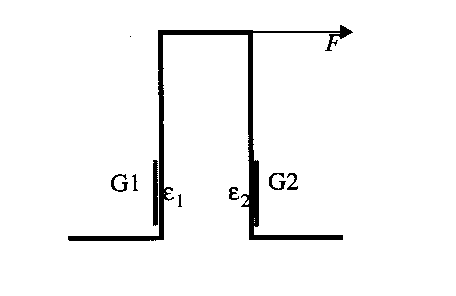
\includegraphics{figs10/00109.eps}}
\caption{ Cantilever beam load cell with gages on either side.	%<!s>
 Strains $\epsilon_1$ and $\epsilon_2$ will be equal and opposite.	%<!s>
 If temperature is same on both sides of beam, we can correct	%<!s>
 for temperature sensitivity.  }	%<!s>
\end{center}
\end{figure}	%<!s>

%%%%** Section 1.6
\paragraph{Wheatstone Bridge}

 Subtraction of the two strain signals is usually accomplished right	%<!s>
 in the load cell itself using a Whetstone Bridge Circuit.	%<!s>
%%%%** Figure 9
\begin{figure}[ht]	%<!s>
\begin{center}
%%\vspace{-1in}
\scalebox{1.2}{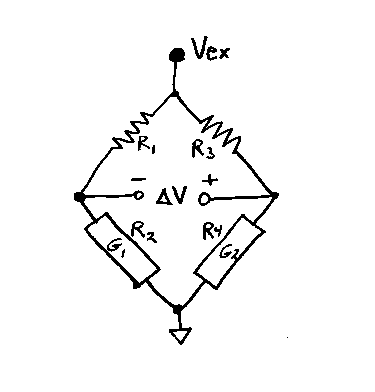
\includegraphics{figs10/00110.eps}}
\caption{ Whetstone Bridge circuit used to subtract resistance	%<!s>
 changes of the two strain gages.  }	%<!s>
\end{center}
\end{figure}	%<!s>

%\end{slide}
%\begin{slide}

A very nice javascript animation illustrating this principle is available at
{\tt http://www.rdpe.com/us/hiw-sglc.htm}.  Be sure to drag the beam tip with your mouse!


Analysis of the bridge circuit yields:
\[
\frac{\Delta V}{V_{ex}} =
\frac{R_4}{R_3 + R_4} - \frac{R_2}{R_1+R_2} =
\frac{R_4R_1 - R_2R_3}{(R_1+R_2)(R_3+R_4)}
\]
%\end{slide}
%\begin{slide}
	%<*hn>
In this example, we place the two strain gages into the bottom legs
of the bridge, ($R_2,R_4$).  The other two legs of the bridge are
non-strain-sensitive resistors (but still temperature sensitive).

	%<*>
We define $\hat{R} = R_0(1+r\Delta T)$.

\[
R_1,R_3 = \hat{R}
\]
\[
R_2 = \hat{R} + (1 + r\Delta T)g R_0 \epsilon_1
\]
\[
R_4 = \hat{R} + (1 + r\Delta T)g R_0 \epsilon_2
\]

From the load cell design, we have $\epsilon_2 = - \epsilon_1$.


%\end{slide}
%\begin{slide}
Computing the output voltage we get:

\[
\frac{\Delta V}{V_{ex}} = \frac{\hat{R}(1+r\Delta T)2gR_0\epsilon_2}
{4\hat{R}^2-(1+r\Delta T)^2 g^2 R_0^2 \epsilon_1^2}
\]


%\end{slide}
%\begin{slide}

Expanding $\hat{R}$ and  canceling terms:

\[
\frac{\Delta V}{V_{ex}} = \frac{2g\epsilon_2}{4-g^2\epsilon_1^2}
\]
Ignoring the high order terms:

\[
\frac{\Delta V}{V_{ex}} = \frac{g\epsilon_2}{2}
\]

Temperature variation is eliminated!  Non-linear term contributes
insignificant errors because $\epsilon$ is very small.

%\end{slide}
%\begin{slide}

%%%%** Section 1.7
\paragraph{Multi-Axis Sensing}
	%<*hn>
In robotics and surgery it is rarely of interest to measure a
single force. In general we want to measure the
	%<*>
6 components of force and torque,

$F_X$

$F_Y$

$F_Z$

$\tau_X$

$\tau_Y$

$\tau_Z$

	%<*hn>
We want to characterize these force/torque
 components at some interface between two
objects.  Examples of these interfaces: robot wrist --- robot hand,
surgical tool handle --- surgical tool body, etc.  So that the sensor
does not distort the forces and torques present, it should be as rigid
as possible.  Therefore the two objects connected by the sensor should
normally be rigidly connected.

Design of load cells for this measurement takes substantial effort
and is beyond the scope of this course. However it is useful
to consider two example designs.

	%<*>
%%%%** Section 1.7.1
\subsubsection{``Maltese Cross'' Sensor}

	%<*hn>
Variations of this design have been produced in a number of
laboratories and are available commercially (Fig. \ref{Maltese}).
In this design,
the spokes of a wheel are instrumented with gages and calibrated
to measure forces and torques applied to the hub relative to the rim.
	%<*>

%<s>\vspace{-3in}
%%%%** Figure 10
\begin{figure}[ht]	%<!s>
\begin{center}
\scalebox{1.0}{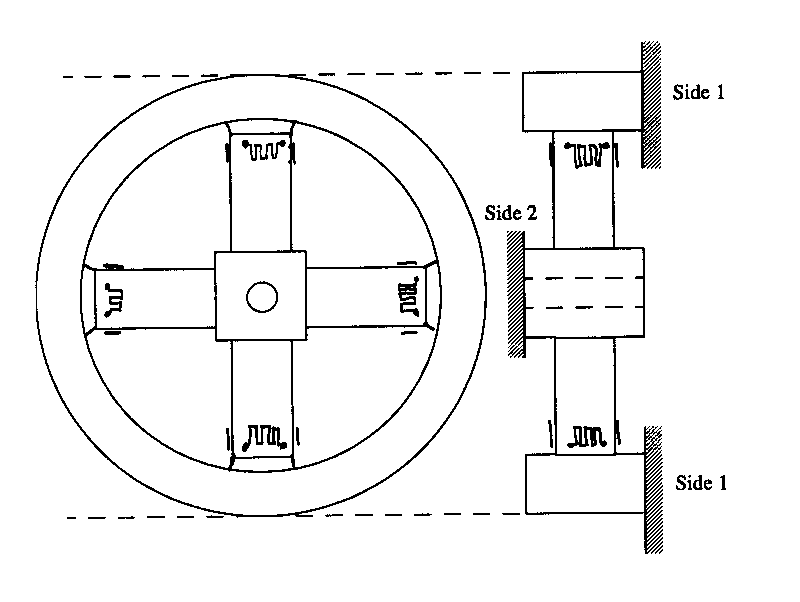
\includegraphics{figs10/00111.eps}}	%<!s>
% \scalebox{0.75}{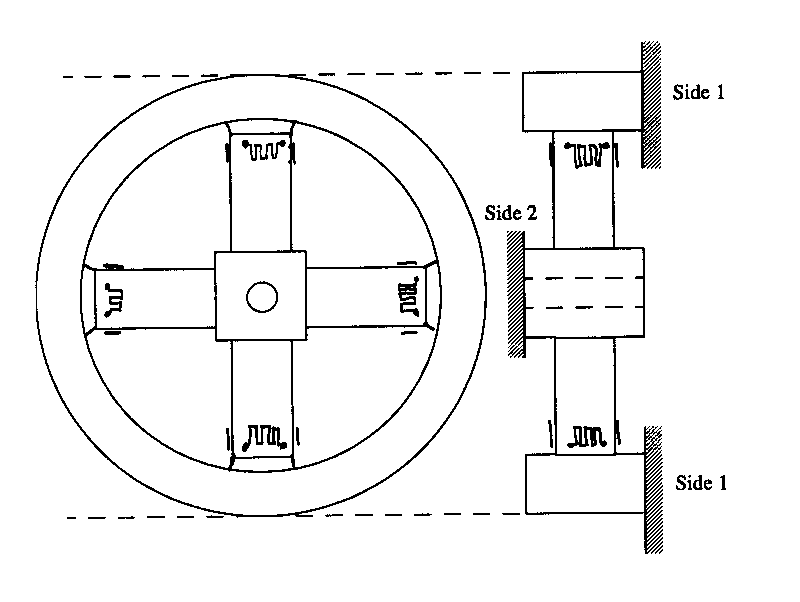
\includegraphics{figs10/00111.eps}}
\caption{ ``Maltese Cross" force-torque sensor.  Forces and	%<!s>
torques applied to the surface labeled `side 1' cause strains in the	%<!s>
spokes which are picked up by 8 attached gages. }\label{Maltese}	%<!s>
\end{center}
\end{figure}	%<!s>

Four gages are applied to each beam for a total of 8 differential
measurements.

A 6x8 calibration matrix C is computed to relate the strain measurements
to forces/torques

%\end{slide}
%\begin{slide}
\[
\left[ \begin{array}{c}
    F_x \\ F_Y \\ F_Z \\ \tau_X \\ \tau_Y \\ \tau_Z
    \end{array}  \right ]
    =
    \left[ \begin{array}{cccccccc}
     & & & & & & &  \\
     & & & & & & &  \\
     & & & C & & & &  \\
     & & & & & & &  \\
     & & & & & & &  \\
     & & & & & & &  \\
     \end{array} \right ]_{6 \times 8}
    \left[ \begin{array}{c}
%    \\ \\ \epsilon \\ \\  \\
    \vspace{0.1in}\\ \\ \epsilon \\ \\\vspace{0.15in}  \\
    \end{array}  \right ]_{8 \times 1}
\]

	%<*hn>
In practice, manufacturing tolerances are not adequate to compute
C from the load cell design with sufficient accuracy
so it must be obtained from measurements of strain outputs as a function
of applied forces and torques for each device using regression
analysis.
	%<*>

%\end{slide}
%\begin{slide}



%%%%** Section 1.7.2
\subsubsection{Parallel-Plate Structure}
	%<*hn>
{\small
(See T. Yoshikawa and T. Miyazaki, ``A six-axis force sensor with
three dimensional cross shape structure," Proc. Intl. Conference
on Robotics and Automation, pp. 249-254, 1989.)
}

An alternative to the bending beam load cell is the parallel plate
structure (also known as a flexure).  In this case, two thin beams
are arranged in parallel (Figure \ref{Parallel}).
	%<*>
%%%%** Figure 11
\begin{figure}[ht]	%<!s>
\begin{center}
\scalebox{1}{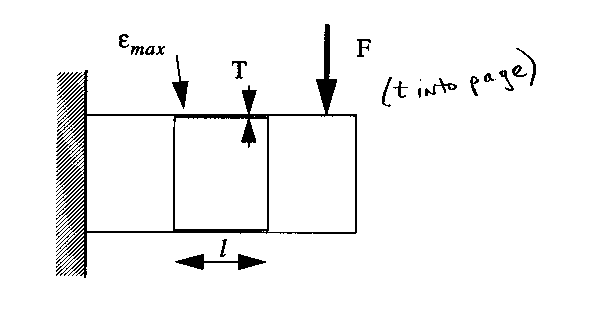
\includegraphics{figs10/00112.eps}}	%<hn>
%\scalebox{1}{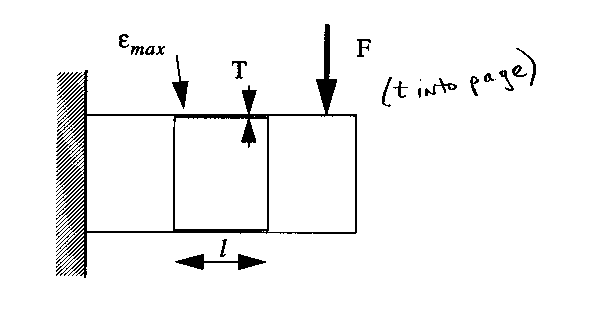
\includegraphics{figs10/00112.eps}}
\caption{ Parallel plate flexure load cell for a single axis.}\label{Parallel}	%<!s>
\end{center}
\end{figure}	%<!s>

%\end{slide}
%\begin{slide}
\paragraph{Analysis}
	%<*hn>
At the point of maximum strain concentration, labeled $\epsilon_{max}$,
the strain is
	%<*>
\[
\epsilon_{max} = \frac{3lF}{\mathrm{E}tT^2}
\]
where t is the width of the parallel plate structure, and E is
Young's Modulus for the material.

%%%%** Section 1.8
\paragraph{Overload Protection}
	%<*hn>
We saw that above a certain critical strain, the ``elastic limit,''
a material will permanently (plastically) deform.  This has two important
consequences. First, if the material deforms plastically, the zero
reading of the load cell will have to be recalibrated. Second, the
load cell will be damaged and will eventually break or suffer reduced
life.

In most realistic force sensing applications, it is difficult or impossible
to predict the maximum forces likely to be experienced by the sensor.
This is because collisions between the sensor and the environment
often occur, either deliberately or as a result of errors. The transient
forces which occur in these collisions (especially with hard objects)
are hard to control and may exceed the design force limit for the sensing
beam.

To prevent damage from these types of events, overload protection is
sometimes designed into force/torque sensors. An overload protection
device must allow safe deflection of the load cell in all active directions
without disturbance forces, but must provide greatly increased stiffness
and strength for deflections above the safe operating point (which may
be a factor of two or more {\it below} the elastic limit.)
%
%\begin{itemize}
%        \item Strains above elastic limit will:
%        \begin{itemize}
%              \item change ``zero'' point of sensor.
%              \item damage or reduce life
%        \end{itemize}
%        \item In realistic applications, hard to predict $F_{max}$
%        \item Overload protection is often required.
%\end{itemize}
	%<*>

%\end{slide}
%\begin{slide}
%<s>\vspace{-1in}
%%%%** Figure 12
\begin{figure}[ht]	%<!s>
\begin{center}
\scalebox{1}{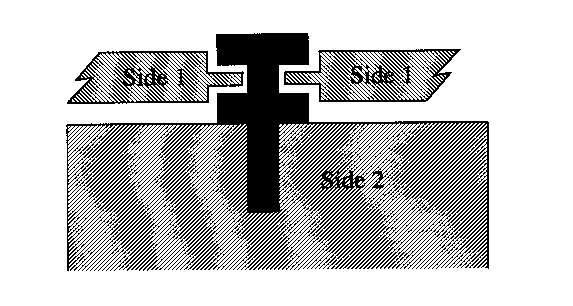
\includegraphics{figs10/00113.eps}}
\caption{ Overload protection scheme for a force/torque sensor.	%<!s>
 a high-strength structural element connects the two sides	%<!s>
 when deflection exceeds the size of its gap to protect the	%<!s>
sensing structure from excessive strain. }\label{Overload}	%<!s>
\end{center}
\end{figure}	%<!s>
	%<*hn>
In the example illustrated in Figure \ref{Overload}, a pin of strong material (i.e.
steel in an aluminum load cell design) is affixed between the two
sides of the load cell so that there is a calibrated gap between the
two sides. When the strain reaches the maximum safe operating point,
the two sides touch and the stiffness of the overall loadcell is greatly
increased.  Once the two sides come into contact through the pin,
the amount of force required to reach the elastic limit is greatly
increased. Any further deflection is thus reduced or eliminated.





\section{Actuators}

\subsection{DC Motors}


\subsubsection{Introduction}

This is a quick overview of DC motors as applied to robot manipulators and
haptic devices.
Although DC motors are a very mature technology, the companies which produce
them are mainly focused on a non-robotics market.   Many commercial applications
are aimed at high velocities and moderate torques.  Robots often require low
velocities and high torques.

The most common way to match available motors to robot needs is to use gears.
A gearbox with ratio $n$ will  reduce motor velocity by $n^{-1}$ and
increase torque by $n$.  Unfortunately, some undesirable properties, such
as the effective inertia of the motor and any friction present in the motor
are increased by $n^2$.   For high performance robotics, including force controlled
robots, teleoperators, and haptic interfaces, these negative effects of gears
are significant and so $n$ must be minimized or made equal to 1.

When $n=1$ in a robotic application, the motor ``sees" a load characterized by
velocities near zero and ``high" torques.   When torques are adequate for the
application motors tend to get hot.  The designer can select among different motors,
but there is a trade-off which cannot be avoided between heat capacity and the
mass of the motor.  Furthermore, large currents can be required which in turn
require large power supplies and thick wires.   Many of the standard techniques
for selecting motors (such as those discussed in motor catalogs) can be too
conservative and result in too much weight for your robot.

 This section explores how to optimize the selection of  a motor for
robotic requirements and how to better understand the thermal behavior of
motors.

\subsubsection{Basic Theory}

DC motors are one of the most common actuators for robotics.
Althought there are many important electric motor technologies for
robot manipulators, here we consider the most basic, brushed DC motors.

Two basic laws   describe the operation of DC motor in terms of
the pair of electrical input variables, $V$ and $I$, and mechanical
output variables, torque, $\tau$ and angular velocity, $\omega$.
\begin{equation}\label{Law1}
\tau = K_m \times I
\end{equation}
\begin{equation}\label{Law2}
V = IR + K_m\omega + L \dot{I}
\end{equation}
where $R$ is the resistance of the armature windings, $K_m$ is the
motor constant\footnote{Note that when MKS units are used there is only one
such constant. When other unit systems are used, two different constants must be used
in the two laws.} and $L$ is the motor inductance.  We will consider
constant currents (i.e. $\dot{I}=0$) and  ignore the
motor inductance.

To illustrate the use of these equations, let us pose some problems:

\begin{figure}
\centering
\scalebox{0.5}{
  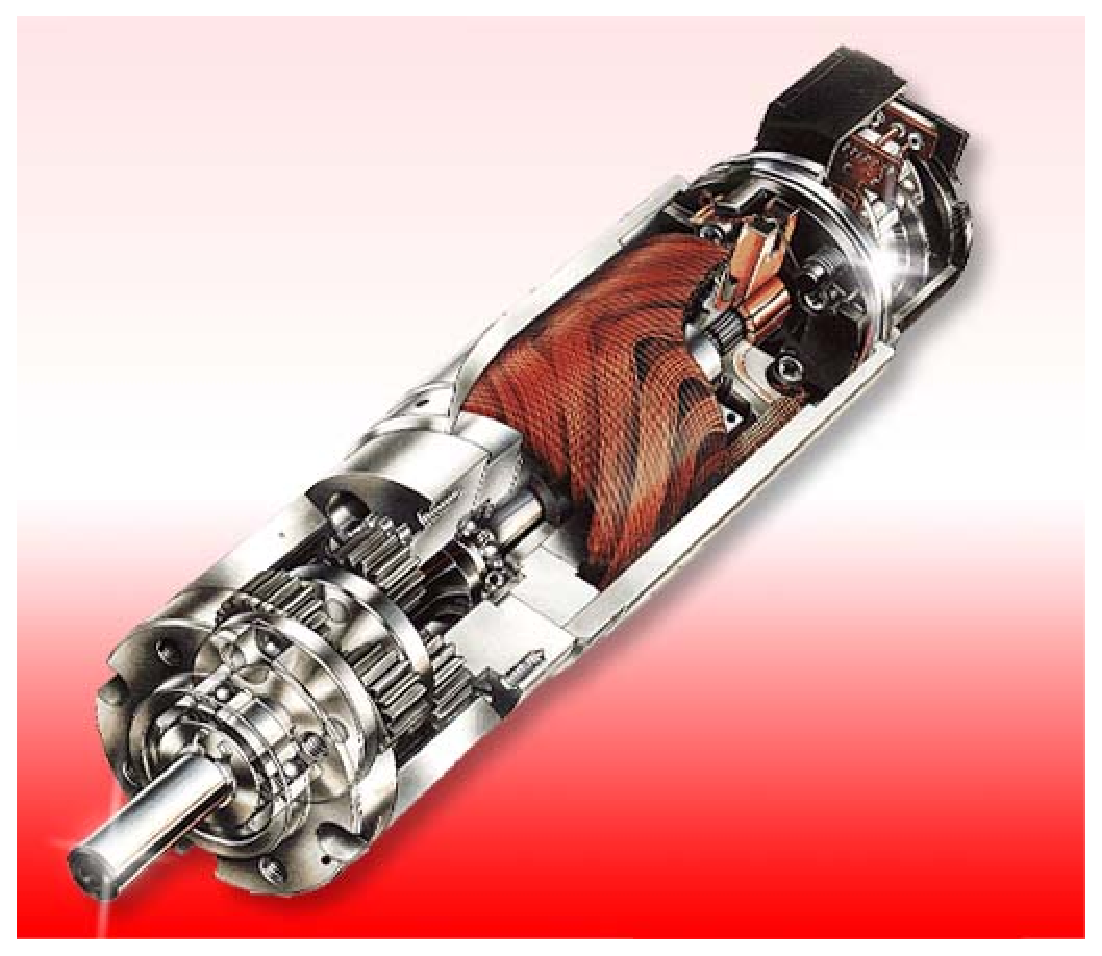
\includegraphics{figs10/motor.eps}
  }
\caption{Maxon brushed DC Motor with gearhead and optical encoder (http://www.maxonmotorusa.com). }
\end{figure}

\subsubsection{Stall Torque}\label{StallProb}
\begin{quotation}
A Maxon RE-25/118752 DC motor\footnote{{\tt http://www.maxonmotorusa.com}} has a motor
constant, $K_m$ of .0234 Nm/A, Coil resistance, $R$ of 2.32 $\Omega$, and winding
inductance, $I$, of 0.24 mH.  In a haptic application, assume $\omega=0$ (this is referred
to as ``stall'').  Assume $\frac{dI}{dt} = 0$. Find the current and voltage required
to generate a torque of 0.05 Nm.
\end{quotation}
{\bf Solution:} Using Equation (\ref{Law1}),
\[
0.05  Nm = 0.0234 Nm/A \times I
\]
\[
I = \frac{0.05}{0.0234} = 2.14A
\]
Using Equation \ref{Law2} for $\omega =0$, we have
\[
V = IR
\]
In other words, for $\omega=0$, the motor acts like a resistor.
\[
V = 2.14A \times 2.32 \Omega + K_M \times 0 + L \times 0
\]
\[
V = 4.96V
\]

\subsubsection{Free Running / Viscous Load}
\begin{quotation}
Using the same motor as in problem \ref{StallProb} find the speed the motor will run with
no load ($\tau = 0$) when 5V is applied.  What will be the current and power dissipation?
Assume $\frac{dI}{dt} = 0$ and that there is no friction in the motor.
\end{quotation}
{\bf Solution:} Using Equation (\ref{Law2}),
\[
5.0V = I\times 2.32 \Omega + 0.0234 Vsec \times \omega
\]
Using Equation (\ref{Law1})
\[
I = 0 (!)
\]
Solving:
\[
\omega = 213.7 rad/sec = 2041 rpm
\]
One way to think about this is that the term $K_m \times \omega$ is a voltage (called
``back EMF") generated internally by the motor which opposes the applied voltage. At no-load,
this voltage exactly cancels the applied voltage and the current is zero.

Since the current is zero, the power is also zero!   This is not
a perpetual motion machine, because
we have assumed there is no friction. Electrical Power in = mechanical power
out:
\[
V\times I = \tau \times \omega = 0
\]


\begin{quotation}
Now, let us consider frictional load to the motor.
The load will be viscous friction with coefficient
$B = 1.2\times 10^{-4} nMsec/rad$. Physically, this
load could be due to 1) the motor's internal
bearing friction and air friction, 2) the friction of
the transmission mechanism such as gears,
belt drives, cable drives, or 3) the external load (such
 as a hole being drilled, drink being
blended, etc).   Find $\omega$, the current, and the power
dissipation when the viscous load
is applied.
\end{quotation}
{\bf Solution:}
The viscous friction load forms another equation which much be solved simultaneously with the
motor equations:
\[
\tau = B\times \omega
\]
Bringing in Equations (\ref{Law2}) and (\ref{Law1}),
\[
5.0V = I\times 2.32\Omega + .0234 \times \omega
\]
\[
\tau = 0.0234\times I
\]
\[
\tau = 1.2\times 10^{-4} \times \omega
\]
\[
I = \frac{1.2\times 10^{-4}}{.0234} \omega \quad = 5.128\times10^{-3}\omega
\]
\[
5.0 = (5.128\times 10^{-3}+ .0234)\omega
\]
\[
\omega = 175.2 rad/sec = 1674 rpm, \quad  I = 0.898A
\]
\[
P = 5.0V\times 0.898A = 4.49 Watts
\]

We can also solve this graphically:


\begin{center}
\scalebox{0.2}{
       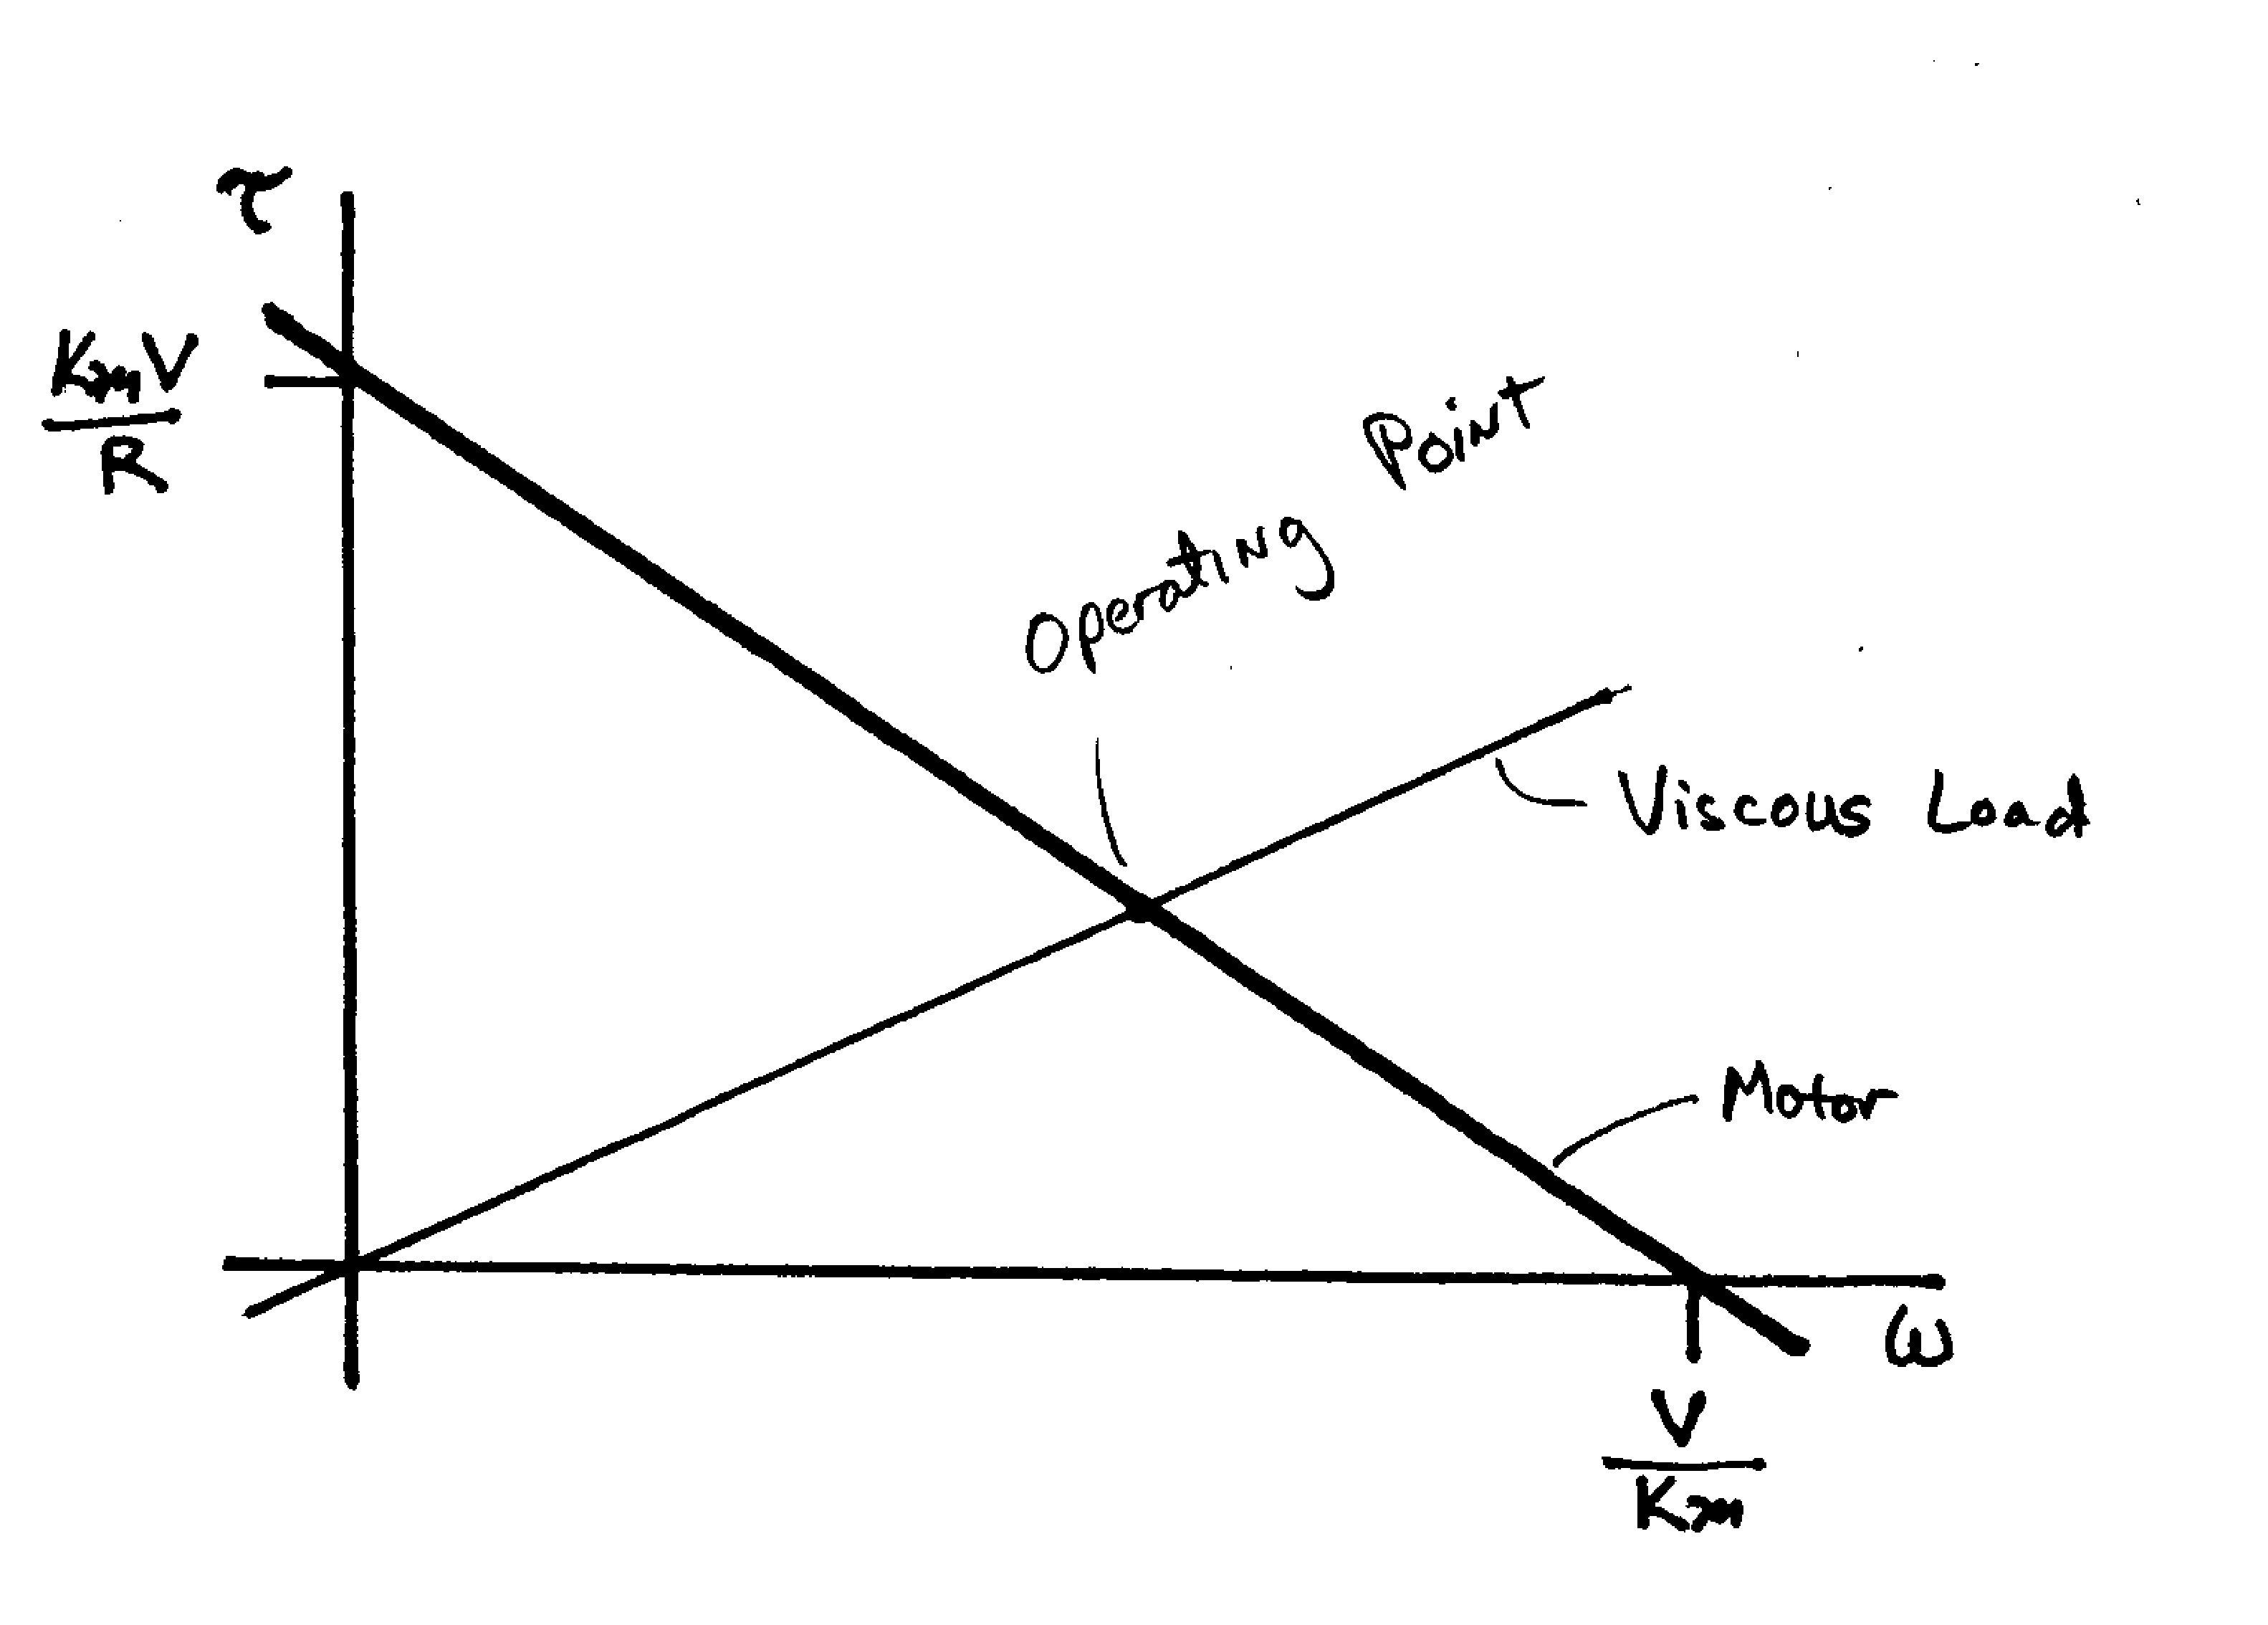
\includegraphics{figs10/00167.eps}
       }
\end{center}


\subsubsection{Power Supply / Winding Selection}
\begin{quotation}
        A DC motor is rated at 150 Watts continuous power (this means that
        the elecrical power cannot exceed 150 Watts in the steady state
        or the coils will burn out).    The manufacturer has a variety of
        150 Watt motors available, each with various values of stall torque
        ($\tau$ when $\omega=0$), coil resistance, motor constant, etc,
        which are listed in a table.
        The manufacturer obtains all these different motors by winding the
        coils with different diameter wire.   For small wire, the number of
        turns which fit into the space is greater (greater $K_m$), but the
        resistance becomes higher.
        We want to use a 30Volt power supply.
        {\bf Problem: } Find the value of $R$ which will give us 150 Watt
        power dissipation at 30V when $\omega =0$.   This way we can get the
        most stall current and therefore the most stall torque.  Find the
        current $I_{max}$ and torque $\tau_{max}$ at 30V.
\end{quotation}

{\bf Solution:}   We want
our 30V power supply to give the maximum permissable
power in this case so:
\[
P = \frac{E^2}{R}
\]
\[
150 = \frac{900}{R}
\]
\[
R = 6\Omega
\]
Now we look through the catalog table for the motor who's coil resistance
is closest to 6$\Omega$.   In this case, the stall current is
\[
I = \frac{30}{6} = 5A
\]
The torque constant for this motor (made up 150W/ 6$\Omega$ motor) is
0.1Nm/A.
\[
\tau_{max} = 0.1 \times 5A = 0.5Nm
\]

\subsubsection{Maximizing Power through duty cycle}

In advanced applications like haptic interfaces, using the motor's continuous power
output can be too conservative.
This is because in haptics the maximum torque output is rarely  needed
100\% of the time.  If we need higher stall torque, we might have to go
up to a motor with a higher wattage rating.  The problem is these can be
very heavy and bulky.  In many haptics applications, this high power capacity
is wasted 90\% of the time.  If we can guarantee that
the peak torque output
(i.e. peak current) will be present for less than 100\% of the time,
we can calculate a higher corresponding electrical power.  If this power
were applied to the motor continuously, it would burn out, but transiently
it will cool off between peaks.     As a rule of thumb, if we can guarantee
an {\it average} torque value is no more than 10\% of the peak, then
we can drive the motor
at a peak power level 10$\times$ its continuous rating.   The percentage of time
that peak current is applied is called the ``duty cycle'' of the application.

So if the motor (and its resistance) is fixed, we need to use a
higher voltage power supply to
get a greater power:
\[
\frac{V^2}{R} = 150\times 10
\]
\[
R = 6\Omega
\]
\[
V = 95V
\]
\[
I_{max} = \frac{95V}{6\Omega} =15.8A
\]
\[
\tau_{max} = 0.1\times 15.8A = 1.58Nm
\]

To summarize, by ASSUMING that the duty cycle is 10\% or less, we can increase
the supply voltage from 30V to 95V and get a peak torque which is 3.16 times
higher.  Since $I_{max}$ increased from 5A to 15.8A, our power supply's peak output
goes from $30V\times5A = 150W$ to $95V\times 15.8A = 1500W$.   So we tripled
peak force output but our power supply cost (proportional to Watts) went up by
a factor of 10!

We must be very careful when using this strategy because if we are wrong
about the average duty cycle, we can burn an expensive motor.


The same duty cycle trick can be used to reduce
the power supply size and cost.
Capacitors can be used to provide the peak current output
required for haptic peaks.   Then the power supply rating can be reduced back
to match the motor's steady state rating.

\newpage

\subsubsection{Thermal Analysis}

In many applications, the ultimate limitation on DC motor performance is
dissipation of heat coming from resistive losses in the motor coils.
When the temperature
gets too high (typically above $180^{\circ}$F) the insulation on the coil wires
melts or burns and the coil shorts out.
The block diagram illustrates the heat generation process from the input of electrical
current, to heat generation in the motor winding (always equal to $I^2R$),
to convective heat transfer out of the motor coils and into the environment.

\begin{center}
\scalebox{.25}{
       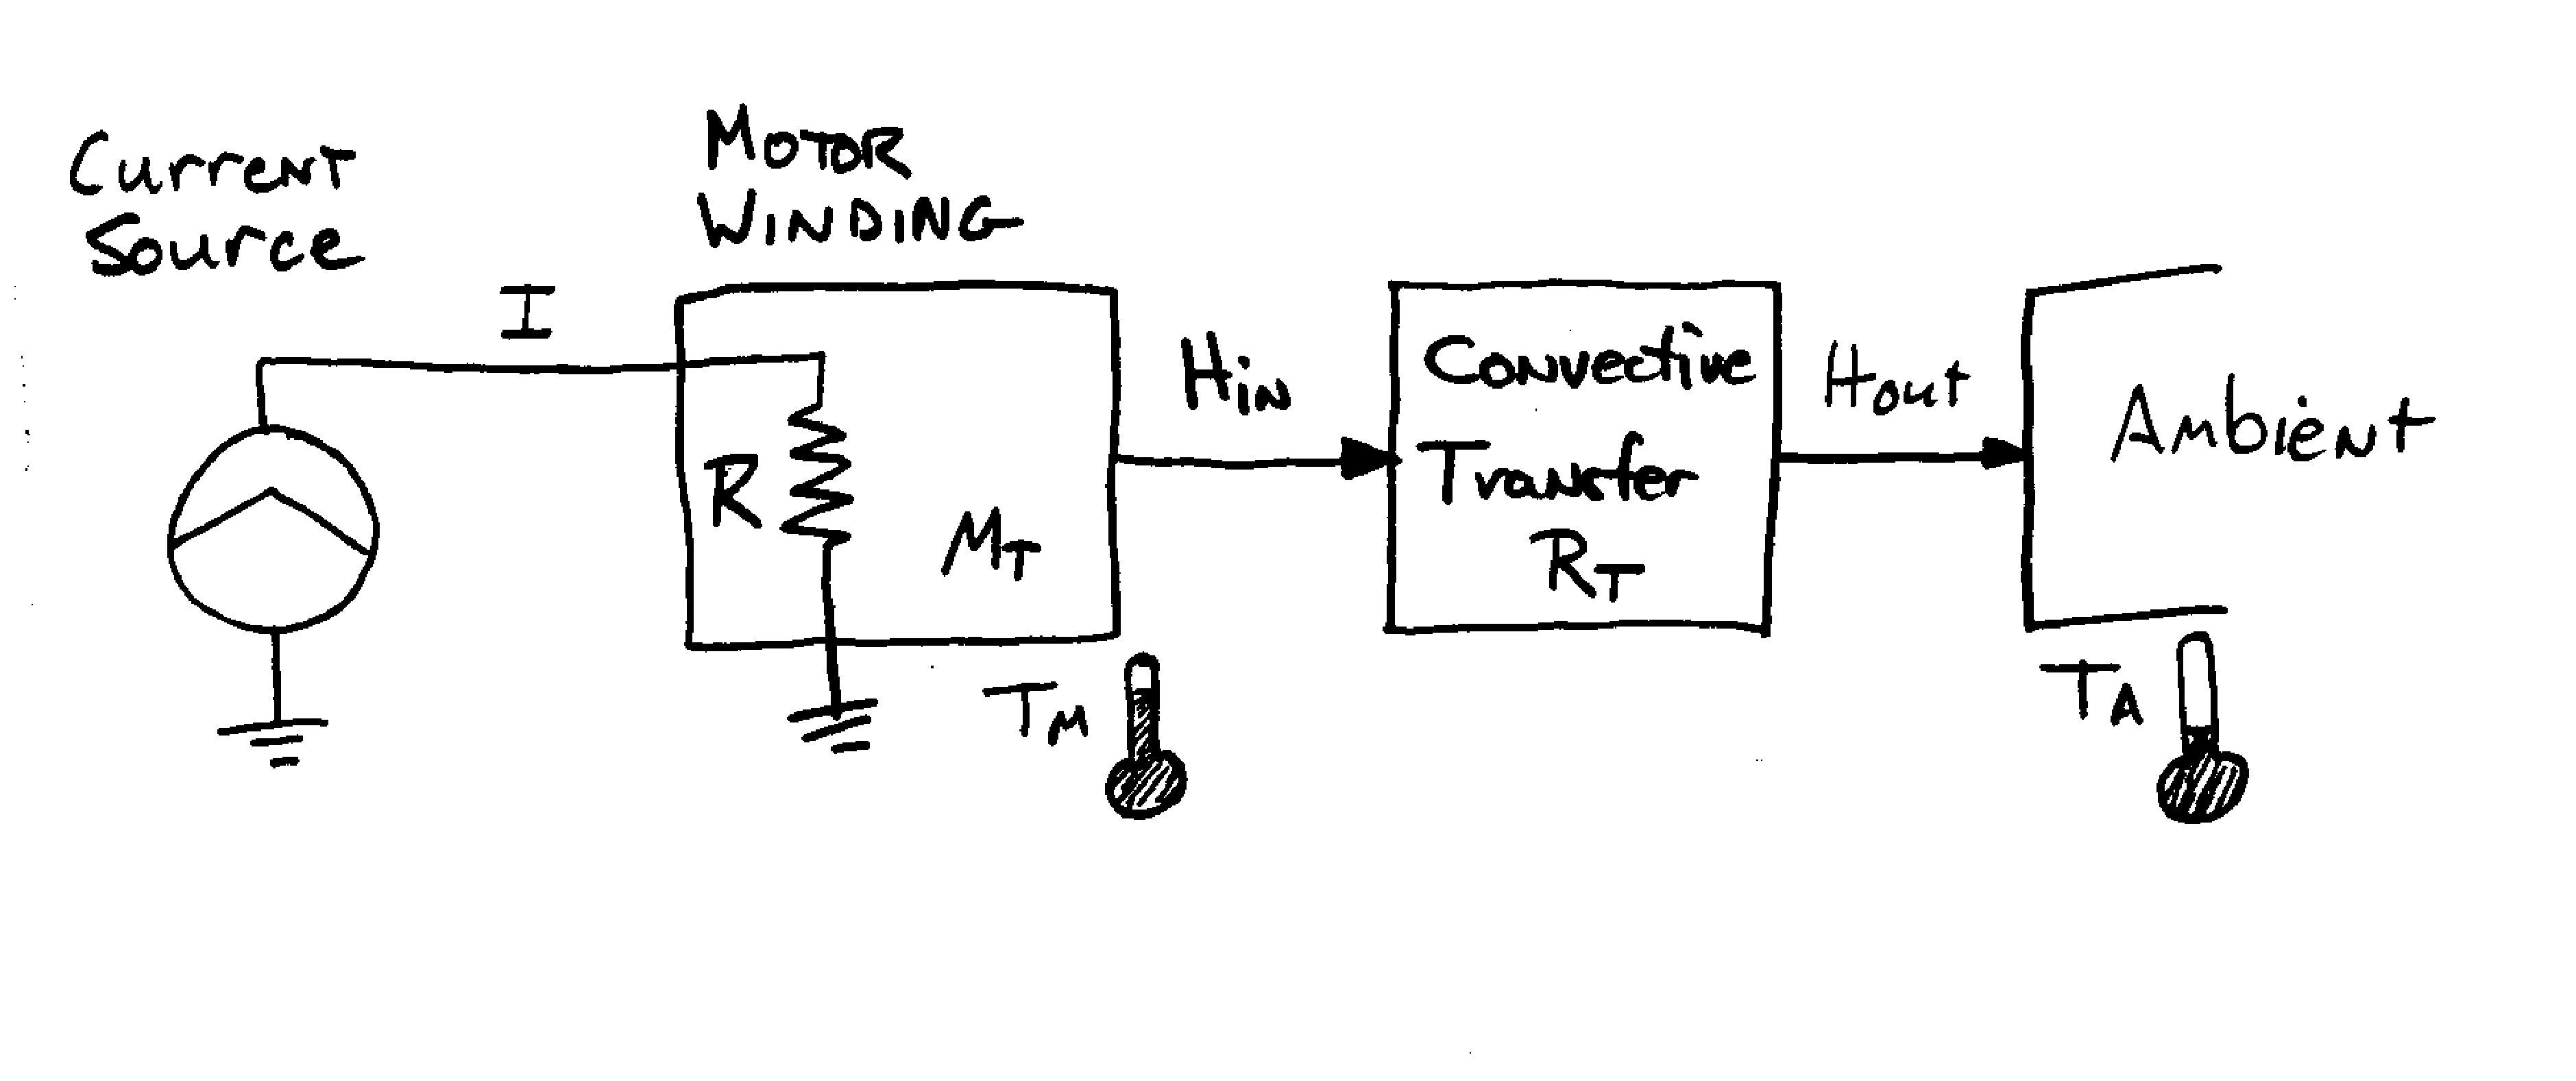
\includegraphics{figs10/00114.eps}
       }
\end{center}


Let us analyze this system:

\subsubsection{}

In robotics we are most likely starting with some algorithm (usually
a control law) which would like to command a certain torque to the
motor.
For a given motor, we need a current
\[
I = \frac{\tau}{K_m}
\]

\subsubsection{}
Heat produced in the coils is always $I^2R$ regardless of $\tau$ and $\omega$.
\[
H_{in} = P = I^2R
\]
We can derive the steady state temperature as a function of $H_{in}$:
\[
T_{in} = P R_T
\]
where $R_T$ is the thermal resistance of the motor (often listed in the
catalog units: $^{\circ}/Watt$).


\subsubsection{}
Heat flows through a thermal resistance in a manner analogous to
current flowing through an electrical resistance.  Temperature plays the
role of voltage.  Thus
\[
H_{out} = \frac{T_M - T_A}{R_T}
\]
where $T_M$ is the motor internal temperature, $T_A$ is the ambient
temperature.

\subsubsection{}
In addition to thermal resistance, objects have a ``thermal mass" which
determines how much thermal energy they can store, and also how fast
temperature builds up when there is a net flow of heat into the object:
\[
T_M = \frac{1}{M_T}\int^t_0 (H_{in} - H_{out}) dt + T_A
\]
where $M_T$ is the thermal mass, and we assume $T_M = T_A$ at $t=0$.

Substituting:

\[
T_M = \frac{1}{M_T}\int^t_0 (P - \frac{T_M - T_A}{R_T} ) dt + T_A
\]
Let $T = T_M - T_A$
\[
T = \frac{1}{M_T}\int^t_0 (P - \frac{T}{R_T} ) dt
\]
Let $\hat{T} = PR_T = I^2RR_T$.  This is the equilibrium temperature if the current
were held constant.
\[
T = \frac{1}{R_TM_T}\int^t_0 (\hat{T}-T ) dt
\]

Taking the LaPlace Transform:
\[
T(s) = \frac{1}{sR_TM_T}(\hat{T}(s) - T(s))
\]

\[
\frac{T(s)}{\hat{T}(s)} = \frac{1}{(1+sR_TM_T)}
\]
Or equivalently:
\[
\frac{T(s)}{I^2(s)} = \frac{RR_T}{(1+sR_TM_T)}
\]

This transfer function describes a thermal system whos input
is current squared (proportional to power) and whos output is
motor temperature.  This system is first order and the time
constant is $R_TR_M$.   Thus our model of motor winding temperature
becomes:

\begin{center}
\scalebox{.25}{
       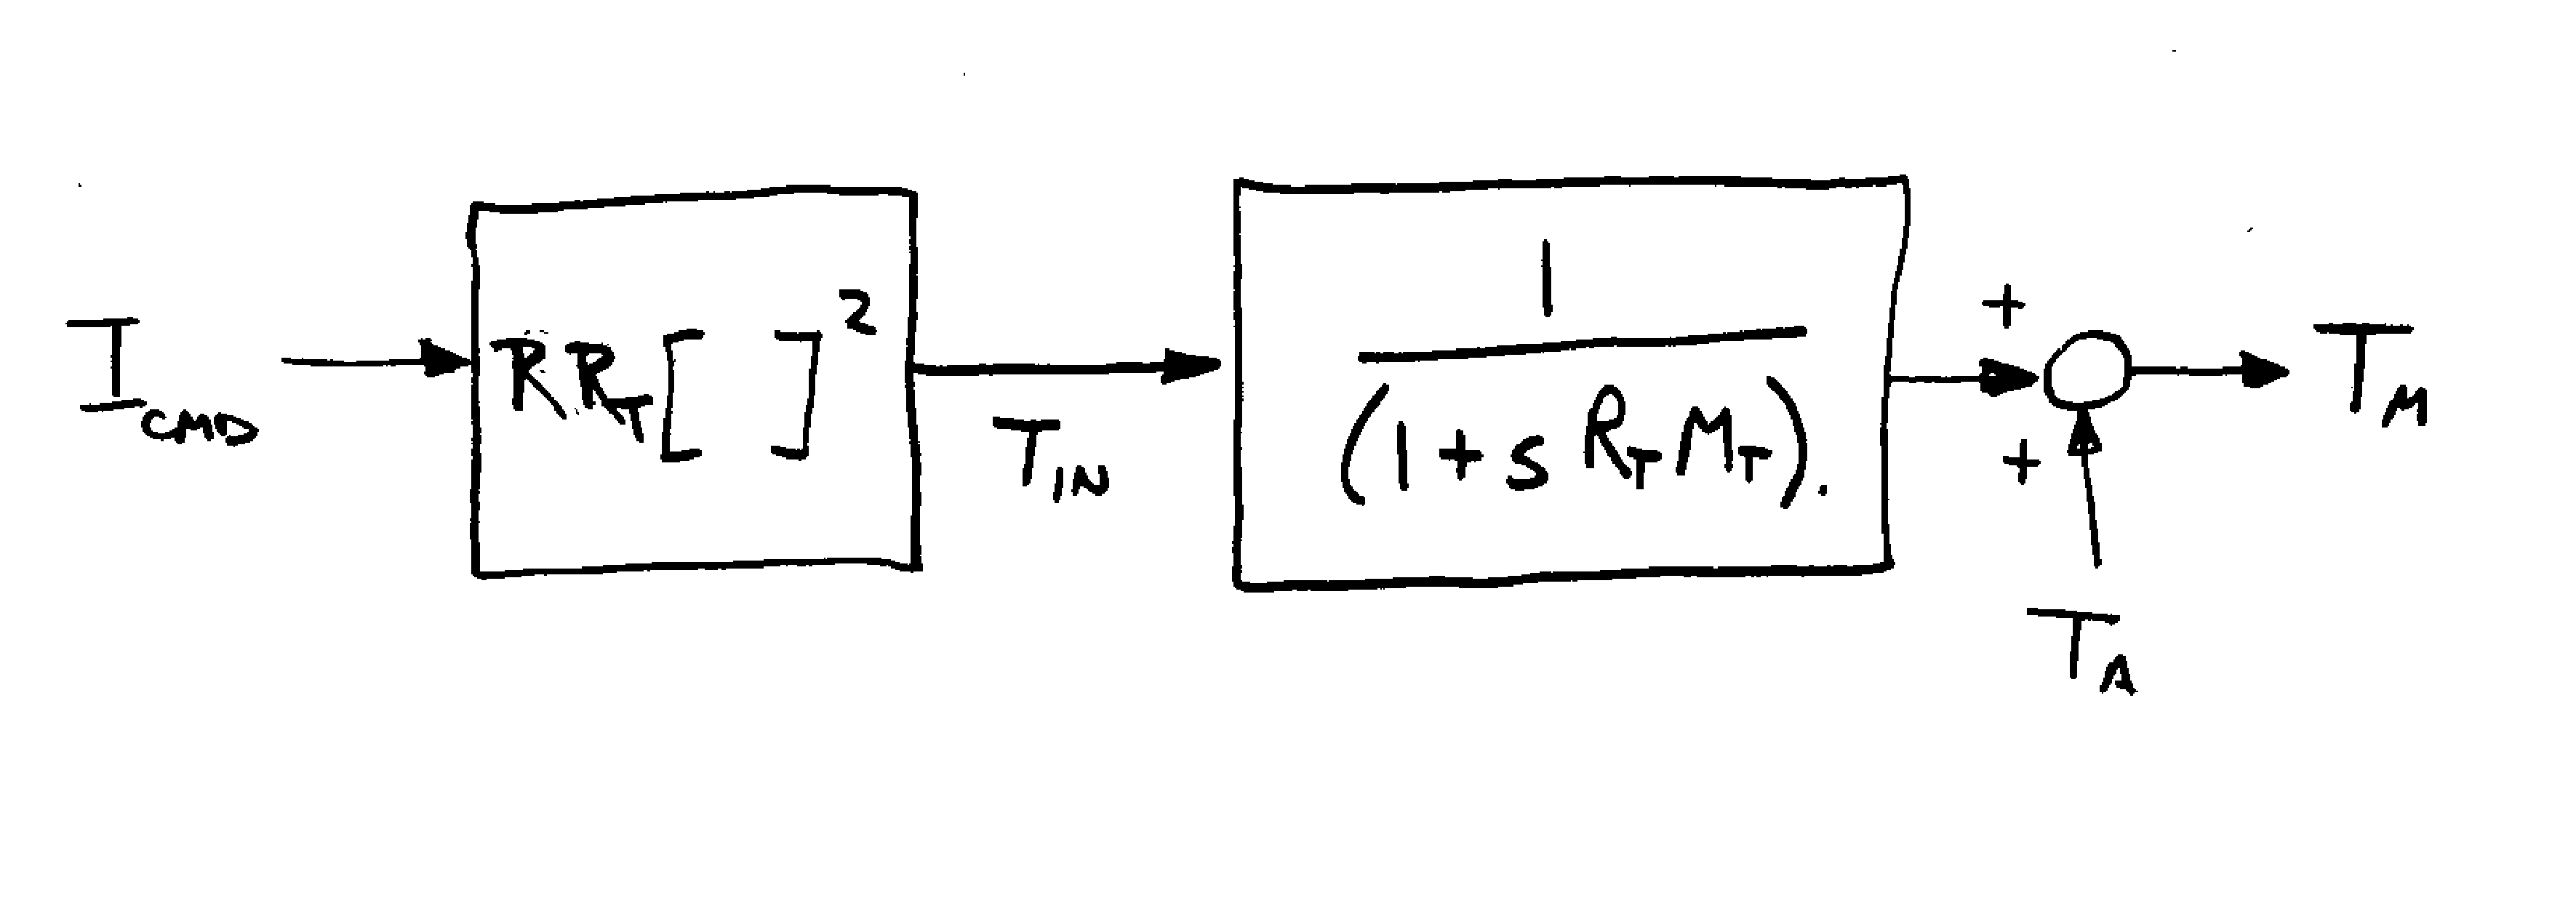
\includegraphics{figs10/00115.eps}
       }
\end{center}

\subsubsection*{Future Material:}

\paragraph{}

[Use of this model to estimate motor winding temperature on-line.
Use of winding temperature sensor to adapt model parameters.]

\paragraph{}

[Real time control of motor current based on measured or estimated
winding temperature.]


\paragraph{}

[Brushed vs. Brushless Motors]








\section{Transmissions}
\section{Joints}
\section{Links}
\section{End Effectors}
\section{Software Architectures}


\section{Summary of Notation}

% Summary of Notation for Chapter  10

